\documentclass[letterpaper]{article}
\usepackage[margin=1in]{geometry}
\usepackage[utf8]{inputenc}
\usepackage{textcomp}
\usepackage{amssymb}
\usepackage{natbib}
\usepackage{graphicx}
\usepackage{gensymb}
\usepackage{amsthm, amsmath, mathtools}
\usepackage[dvipsnames]{xcolor}
\usepackage{enumerate}
\usepackage{mdframed}
\usepackage[most]{tcolorbox}
\usepackage{csquotes}
% https://tex.stackexchange.com/questions/13506/how-to-continue-the-framed-text-box-on-multiple-pages

\tcbuselibrary{theorems}

\newcommand{\R}{\mathbb{R}}
\newcommand{\Z}{\mathbb{Z}}
\newcommand{\N}{\mathbb{N}}
\newcommand{\Q}{\mathbb{Q}}
\newcommand{\C}{\mathbb{C}}
\newcommand{\code}[1]{\texttt{#1}}
\newcommand{\mdiamond}{$\diamondsuit$}
\newcommand{\PowerSet}{\mathcal{P}}
\newcommand{\Mod}[1]{\ (\mathrm{mod}\ #1)}
\DeclareMathOperator{\lcm}{lcm}

%\newtheorem*{theorem}{Theorem}
%\newtheorem*{definition}{Definition}
%\newtheorem*{corollary}{Corollary}
%\newtheorem*{lemma}{Lemma}
\newtheorem*{proposition}{Proposition}


\newtcbtheorem[number within=section]{theorem}{Theorem}
{colback=green!5,colframe=green!35!black,fonttitle=\bfseries}{th}

\newtcbtheorem[number within=section]{definition}{Definition}
{colback=blue!5,colframe=blue!35!black,fonttitle=\bfseries}{def}

\newtcbtheorem[number within=section]{corollary}{Corollary}
{colback=yellow!5,colframe=yellow!35!black,fonttitle=\bfseries}{cor}

\newtcbtheorem[number within=section]{lemma}{Lemma}
{colback=red!5,colframe=red!35!black,fonttitle=\bfseries}{lem}

\newtcbtheorem[number within=section]{example}{Example}
{colback=white!5,colframe=white!35!black,fonttitle=\bfseries}{def}

\newtcbtheorem[number within=section]{note}{Important Note}{
        enhanced,
        sharp corners,
        attach boxed title to top left={
            xshift=-1mm,
            yshift=-5mm,
            yshifttext=-1mm
        },
        top=1.5em,
        colback=white,
        colframe=black,
        fonttitle=\bfseries,
        boxed title style={
            sharp corners,
            size=small,
            colback=red!75!black,
            colframe=red!75!black,
        } 
    }{impnote}
\usepackage[utf8]{inputenc}
\usepackage[english]{babel}
\usepackage{fancyhdr}
\usepackage[hidelinks]{hyperref}

\pagestyle{fancy}
\fancyhf{}
\rhead{CSE 101}
\chead{Wednesday, March 2, 2022}
\lhead{Lecture 22}
\rfoot{\thepage}

\setlength{\parindent}{0pt}

\begin{document}

\section{NP-Completeness}
For almost every problem that we've seen in this class, there's a (usually bad) naive algorithm that just considers every possible answer and returns the best one. Some examples are: 
\begin{itemize}
    \item What is the shortest path from $s$ to $t$ in $G$? 
    \item What is the longest common subsequence? 
    \item What is the cloest pair of points? 
    \item Does $G$ have a topological ordering?
\end{itemize}
Of course, for nearly every algorithm we've discussed in class thus far, we were able to come up with a clever solution that runs in polynomial time. However, it's not generally the case that such (clever) algorithms will exist. 

\bigskip 

Note that, in this class, we define an \emph{easy} problem to be one that can be solved in polynomial time and a \emph{hard} problem to be one that cannot be solved in polynomial time. 

\subsection{Nondeterministic Polynomial (NP)}
Such problems are said to be in \textbf{Nondeterministic Polynomial} time (NP). To think of this in a theoretical perspective, imagine some nondeterministic computer that can try every possibility in parallel and then return the best possible solution. This type of computer can solve these problems in polynomial time. For example, it is allowed to search for the shortest path by trying every single path in \emph{parallel} and seeing which one is the shortest. There are two types of NP problems.
\begin{itemize}
    \item \textbf{NP-Decision} problems ask if there is some object that satisfies a polynomial time-checkable property. For example, is there a path from $s$ to $t$? If you write down a path from $s$ to $t$, then it is easy for the computer to check, in polynomial time, whether this is actually a valid path from $s$ to $t$. So, effectively, a decision problem is one whose answer is either \underline{yes} or \underline{no}.
    \item \textbf{NP-Optimization} problems ask for the object that maximizes (or minimizes) some polynomial time-computable objective. For example, instead of asking if there is a path from $s$ to $t$, you might instead ask what the shortest path from $s$ to $t$ is. So, effectively, an optimization problem is one whose answer is a minimum or maximum value. 
\end{itemize}
Essentially, $NP$ is the set of problems for which you can \emph{verify} the answer in polynomial time. Alternatively, it's the set of problems that can be solved in polynomial time by a \emph{nondeterministic} computer. 

\subsection{Difference Between Decision \& Optimization Problems}
% TODO expand on this
Now, note that NP-Decision and NP-Optimization problems are not too different. 
\begin{itemize}
    \item Every decision problem can be phrased as an optimization problem.
    \item Every optimization problem has a decision form.
\end{itemize}
For theoretical reasons, it's a good idea to understand the distinction. But, for practical purposes, it doesn't really matter. 

\subsection{Examples of NP Problems}
Some examples of NP problems are: 
\begin{itemize}
    \item Formula-SAT (NP-Decision). 
    \item Traveling Salesman Problem (NP-Optimization). 
    \item Hamiltonian Cycles (NP-Decision). 
    \item Generalized Knapsack (NP-Optimization). 
    \item Maximum Independent Set (NP-Optimization). 
\end{itemize}

\subsubsection{Formula-SAT}
Given a logical formula in a number of Boolean variables, is there an assignment to the variables that causes the formula to be true? 

\bigskip

For example, consider the following formulas: 
\begin{itemize}
    \item \underline{Formula 1:} If $x = \text{True}$, $y = \text{True}$, and $z = \text{False}$, then the following formula is satisfied: 
    \[(x \lor y) \land (y \lor z) \land (z \lor x) \land (\overline{x} \lor \overline{y} \lor \overline{z})\]

    \item \underline{Formula 2:} No assignments of $x$, $y$, and $z$ can satisfy the following formula: 
    \[(x \lor y) \land (y \lor z) \land (z \lor x) \land (\overline{x} \lor \overline{y}) \land (\overline{y} \lor \overline{z}) \land (\overline{x} \lor \overline{z})\]
\end{itemize}
There are some applications of SAT. In particular: 
\begin{itemize}
    \item \underline{Circuit Design:} Given some circuit, you want to make sure it actually computes the function that it's supposed to compute. This is basically a satisfiability problem.
    \item \underline{Logic Puzzle:} Most logic puzzle usually come down to some satisfiability problem; you want to find some settings or variables that satisfy some set of rules. 
\end{itemize}


\subsubsection{Hamiltonian Cycles}
Given an undirected graph $G$, is there a cycle that can visit every vertex exactly once? 

\subsubsection{General Knapsack}
\emph{Recall} that knapsack has a number of items, each with a weight and a value. The goal is to find the set of items whose total value is as much as possible without the total weight exceeding some capacity. 

\bigskip 

The general knapsack problem essentially runs in polynomial time in the \emph{weights}. Note that if the weights are allowed to be large (for example, written in binary), then you don't have a good algorithm. 


\subsection{Brute-Force Search}
Every NP problem has a brute-force search algorithm (the naive algorithm). In this class, we have looked at problems with algorithms that substantially improve on these brute-force algorithms. The question, then, is: \emph{does every NP problem have a better-than-brute-force algorithm?} Put it another way, \emph{is it the case that every algorithm in NP has a polynomial time algorithm?} 
\begin{itemize}
    \item If this is the case, then every NP problem has a reasonably efficient solution. No matter what kind of complicated search or decision problem we want to solve, there is always a clever way to do it better than brute-force. 
    \item If this is \emph{not} the case, then some NP problems are fundamentally difficult. There are some problems which are easy to check but there is no straight-forward or efficient way to actually find the answer.  
\end{itemize}
Note that $P$ is the set of all problems that can be solved in polynomial time. 

\subsection{Reductions}
In practice, at least some problems in NP appear to be hard. Despite decades of trying, people still don't know particularly good problems. Suppose you have a problem. How do you know if it's hard or not? 
\begin{itemize}
    \item You can search for an efficient algorithm to show that the problem is easy.
    \item You can try to prove that the problem is hard, but this is difficult. 
    \item You can try to relate the difficulty of your problem to the difficult of other problems.
\end{itemize}
With the last bullet point, we'll introduce the notion of \emph{reductions}. 

\subsubsection{What Is It?}
Reductions are a method for proving that one problem is \emph{at least as hard} as another problem. You can think of this as proving inequalities about problems. For example, problem $A$ is as hard as problem $B$. 

\bigskip 

The way we do this is as follows: we can show that \emph{if} there is an algorithm for solving $A$, then we can use this algorithm to solve $B$. Therefore, $B$ is no harder than $A$. 

\bigskip 

To better understand this concept, consider the following statements:
\begin{itemize}
    \item If problem $X$ is no harder than problem $Y$, and if $Y$ is easy, then $X$ must also be easy. 
    \begin{mdframed}[]
        To get the intuition behind this, suppose you have two numbers $x$ and $y$ such that $x$ is no greater than $y$; that is, $x \leq y$. Suppose $y$ is negative. Then, $x$ must also be negative (it cannot be positive). 

        \bigskip 

        The same idea holds here. If we have two problems $X$ and $Y$ such that $X$ is no harder than (or at least as easy as) $Y$ and $Y$ is easy, then $X$ cannot be harder than $Y$; $X$ has to be \emph{as easy as, or easier than,} $Y$. 
    \end{mdframed}
    \item If problem $X$ is no harder than problem $Y$, and if $X$ is hard, then $Y$ must also be hard. 
    \begin{mdframed}[]
        Again, to get the intuition behind this, suppose you have two numbers $x$ and $y$ such that $x$ is no greater than $y$; that is, $x \leq y$. Suppose $x$ is positive. Then, $y$ must also be positive (it cannot be negative). 

        \bigskip 

        The same idea holds here. If we have two problems $X$ and $Y$ such that $X$ is no harder than (or at least as easy as) $Y$ and $X$ is hard, then $Y$ cannot be easier than $X$; $Y$ has to be \emph{as hard as, or harder than,} $X$. 
    \end{mdframed}
\end{itemize}



\subsubsection{Reducing Hamiltonian Cycle to Traveling Salesman Problem}
We note that there is a natural reduction here. Particularly, they're related in the sense that we're visiting each vertex exactly once. 
\begin{itemize}
    \item Recall that the Traveling Salesman Problem asked: \emph{Given a weighted (undirected) graph $G$ with $n$ vertices, find a cycle that visits each vertex exactly once whose total weight is as small as possible.}
    \item Recall that the Hamiltonian Path problem asked: \emph{Given an undirected graph $G$, is there a cycle that can visit every vertex exactly once?}
\end{itemize}
To see this in action, consider the following example: 
\begin{center}
    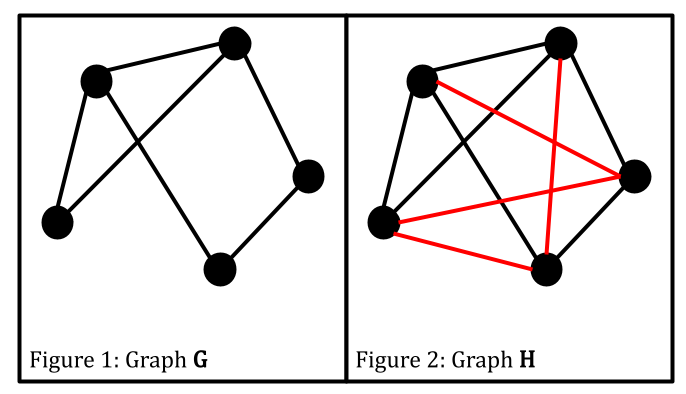
\includegraphics[scale=0.4]{../assets/ham_tsp.png}
\end{center}
Suppose we have an algorithm that solves the Traveling Salesman Problem efficiently. The idea is to convert a Hamiltonian Cycle problem to a Traveling Salesman problem. We do this by taking the original graph $G$ from the Hamiltonian Cycle problem and ``copying'' it to the Traveling Salesman problem, which we'll call the copied graph $H$. For all edges in $G$, we can give the corresponding edges in $H$ a weight of 1 (in Figure 1 and 2, the \emph{black} edges). Then, any extra edges that we add to $H$ (in Figure 2, the \emph{red} edges) can be given a very expensive weight (say 1000). 
\begin{center}
    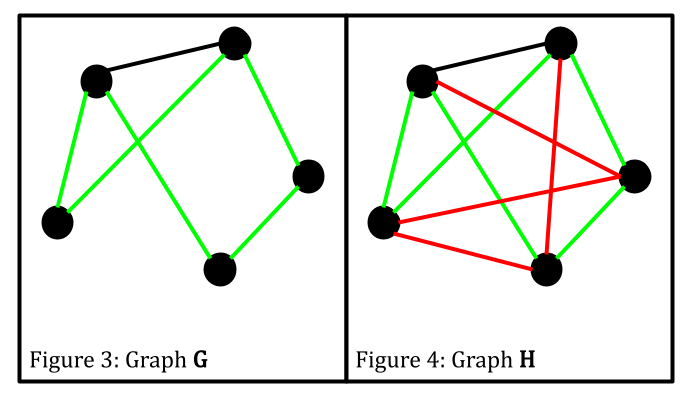
\includegraphics[scale=0.4]{../assets/ham_tsp_2.png}
\end{center}
Looking at Figure 4, we see that there is a Traveling Salesman path of cost 5. But, the path taken in the Traveling Salesman problem is the same path found in the Hamiltonian Cycle problem. So, the cheapest path we can hope for in the Traveling Salesman problem is the path consisting only of cost 1 edges. So, if we can find a path in the Traveling Salesman problem consisting only of cost 1 edges, then we have a Hamiltonian Cycle. \emph{Otherwise}, we'll have to make use of some expensive edges, so that implies that no such Hamiltonian Cycle can exist. 


\bigskip 

To be more formal about it, suppose you have a Hamiltonian Cycle instance $G$ with $n$ vertices. Suppose that you have an efficient algorithm $A$ that solves the Traveling Salesman Problem\footnote{We don't need to know how this algorithm works, only that you \emph{have} one.} Now, we create a Traveling Salesman problem instance $H$ where: 
\begin{itemize}
    \item The edges in $G$ have cost 1. 
    \item The edges not in $G$ have cost 1000 (or some expensive weight). 
\end{itemize}
Then, using this Traveling Salesman Problem algorithm, we can solve the Traveling Salesman instance. We note that we have a path of cost $n$ in $H$ if and only if there is a Hamiltonian cycle in $G$. Therefore, we can use this answer to solve the initial problem. 
\begin{itemize}
    \item If there is a Hamiltonian Cycle in $G$, then the Traveling Salesman Problem will have a weight of $n$. If there is \emph{no} Hamiltonian Cycle, then the best cost will be greater than $n$. 
    \item Any Traveling Salesman Problem that uses these expensive-costing edges will be more expensive than if we decided to use the edges with cost 1. 
    \item Therefore, we can run $A(H)$. If $A(H) \leq n$, then $G$ has a Hamiltonian cycle. Otherwise, it does not. 
\end{itemize}
From this, we get a new algorithm that can solve the Hamiltonian Cycle. This gives us a relation: the Hamiltonian Cycle problem is \emph{no harder} than the Traveling Salesman Problem. Now, since Hamiltonian Cycle is in NP, then it follows that the Traveling Salesman Problem must also be in NP. 

\bigskip 

So, what we've shown is that if we have an algorithm that can solve the Traveling Salesman problem, then we can turn that into an algorithm that solves the Hamiltonian Cycle path. 

\subsubsection{Generalization}
If we want to find a reduction from problem $A$ to problem $B$, then what we want to show is: 
\begin{itemize}
    \item If we are given an algorithm to solve that solves problem $B$, we can turn that into an algorithm that solves problem $A$. 
    \item Generally, we start with an instance of problem $A$. Then, with some polynomial time reduction algorithm, we can turn this instance of problem $A$ into an instance of problem $B$. Then, with a \emph{hypothetical} algorithm for problem $B$, we can find a solution to the problem $B$ instance. Then, we need to turn this solution of the problem $B$ instance into a solution for the problem $A$ instance; this is done by using a polynomial time interpretation algorithm. 
\end{itemize}
This process looks something like: 
\begin{center}
    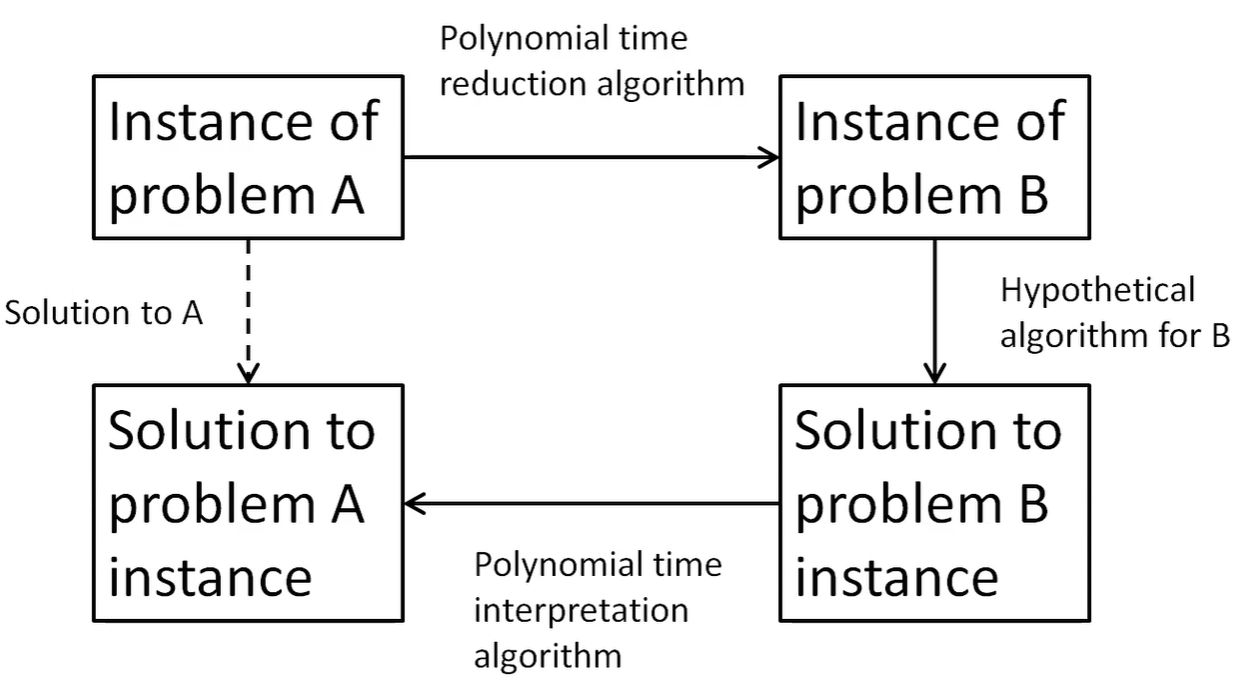
\includegraphics[scale=0.4]{../assets/reduction_cycle.png}
\end{center}
It's important that the reduction and interpretation algorithms run in \emph{polynomial time} by construction. If you have a polynomial time algorithm for problem $B$, then this entire process runs in polynomial time (i.e. you have a polynomial time algorithm for problem $A$). If you don't have a polynomial time algorithm for problem $B$, then there might be some other way to solve problem $A$, but you can't use this particular method. 

\bigskip 

So, effectively, if we have algorithms for reduction and interpretation, then: 
\begin{itemize}
    \item Given an algorithm to solve problem $B$, we can turn it into an algorithm to solve problem $A$. 
    \item This means that problem $A$ might be \emph{easier} to solve than problem $B$, but it cannot be \emph{harder}.
\end{itemize}

\end{document}